
\documentclass[12pt]{article}
\usepackage{wrapfig}
\usepackage{siunitx}
\usepackage[utf8]{inputenc}
\usepackage[english]{babel}
\usepackage{graphicx}
\usepackage{hyperref}
\usepackage{xcolor}
\hypersetup{
    colorlinks=true,
    linkcolor=black,
    filecolor=black,
    urlcolor=cyan,
}
\urlstyle{same}
\author{{\Huge Carl Jonas Mikaelsson Berggren}}
\font\myfont=cmr12 at 30pt
\title{{\myfont Spezielle Relativität}}

\begin{document}
\maketitle
\tableofcontents
\newpage
\begin{abstract}
In diesem Dokument erkläre ich, wie ich ein Programm entwickelt habe, was Albert Einsteins spezielle Relativität visualisiert.
Das Programm arbeitet anhand von Minkowski-Raumzeitdiagrammen, und nutzt objektorientierte Programmierung.

Außerdem erkläre ich die darunter liegende Physik, und leite den Lorentz-Faktor her.
Dabei werde ich auf Relativität vor Einstein, auf die Funktionsweise von Minkowski-Raumzeitdiagrammen, auf die Transformationen zwischen Bezugssystemen, auf Vierervektoren, auf die Implikation spezieller Relativität, und dessen Einschränkungen eingehen.
Dabei beziehe ich mich nur auf spezielle Relativität und nehme Inertialsysteme in einer flachen Raumzeit an.
\end{abstract}
\section{Relativität nach Newtonscher Physik}
Bevor wir über Einsteins spezielle Relativität reden können, müssen wir das Konzept von Raum, Zeit und Bewegung klarstellen.
\subsection{Bezugssysteme}
Zunächst muss klar gestellt werden, wie Position, Zeit und Geschwindigkeit gemessen werden.
Dazu muss ein Koordinatensystem räumlich und zeitlich definiert werden.
Das Koordinatensystem hat einen Ursprung  mit $x = y = z = t = 0$.
Hierbei liegt der Ursprung, des Koordinatensystems, in der Regel auf einem Objekt zu Beginn des Beobachtungszeitraums.
Durch die Tatsache, dass in allen Inertialsystemen die gleichen physikalischen Gesetze gelten, sind alle Bezugssysteme gleichermaßen gültig.
Es ist keine universal-gültige Aussage über die Position oder Geschwindigkeit eines Körpers, oder Zeitpunkt eines Ereignisses möglich.
Demnach ist es bedeutungslos zu sagen, man hätte zum Zeitpunkt $t$ die Position $x, y, z$ und bewege sich mit einer Geschwindigkeit $\vec{v}$.
Es muss immer ein bekannter Bezugspunkt gewählt werden: z.b. Erdmittelpunkt, Upload des ersten http Dokuments.
Bezugssysteme können sich also relativ zu einander bewegen, und dennoch gleichermaßen gültig, das selbe Ereignis beschreiben.
\subsection{Galilei-Transformation}
Ich werde mich im folgenden auf eine Raumdimension beschränken.
Weitere Raumdimensionen können hinzugefügt werden, indem die gerichteten Größen durch Vektoren ersetzt werden.
$x$ wird demnach zu $\vec{0p}$ und $v$ zu $\vec{v}$.
Dabei ist zu beachten, dass die gerichteten relativistischen Effekte nur endlang der Bewegungsrichtung auftreten.
Wie dies funktioniert wird in Abschnitt \ref{4v} näher erläutert.

Es wird zunächst ein Bezugssystem gewählt, mit den Größen $x, t$ und $v$.
Anschließend wird ein gestrichenes Bezugssystem gewählt mit den Größen $x', t'$ und $v'$, wobei $t = t'$ gilt.
Aus unserer alltäglichen Erfahrung geht hervor, dass für die Position eines, zu dem ungestrichenen System, statischen Objekts gilt:
\begin{equation}
x' = x-vt
\end{equation}
Genau so gilt für Geschwindigkeiten:
\begin{equation}
\label{vnewton}
u' =u - v
\end{equation}
Hierbei ist v die Geschwindigkeit des gestrichenen Bezugssystems und $u$ Die Geschwindigkeit des betrachteten Objekts.

\begin{wrapfigure}{R}{0.4\textwidth}
\centering
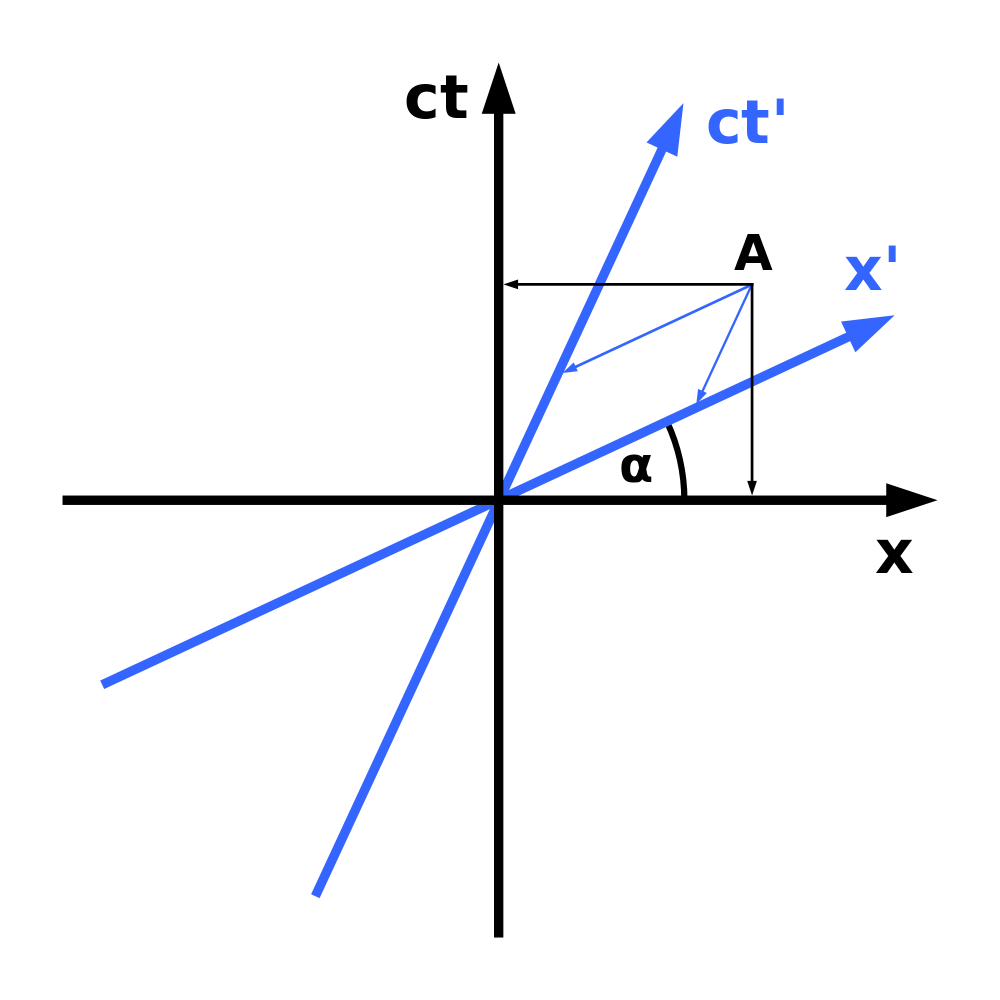
\includegraphics[width=0.3\textwidth]{Minkowski_diagram.png}
\end{wrapfigure}
\subsection{Minkowsky-Raumzeitdiagramme}
Das Minkowski-Raumzeitdiagramm betrachtet, in seiner üblichen Form, Objekte in einer Raumdimension und Zeit.
Hierzu wird die Zeit auf die vertikale Achse gelegt und die Position auf die horizontale.
Für die Betrachtung von spezieller Relativität, werden die Einheiten einfachheitshalber so gewählt, dass für die Lichtgeschwindigkeit $c = 1$ und für
die Position $x = ct$ gelten.
Objekte werden als Geraden dargestellt und Ereignisse als Punkte.
Durch die Wahl der Einheiten, wird Licht somit als diagonale Gerade dargestellt.
\newpage
\section{spezielle Relativität}
Die spezielle Relativität fügt ein entscheidendes Postulat hinzu:
\begin{itemize}
\item Die Lichtgeschwindigkeit ist ein universelle Konstante
\end{itemize}
Dies wirft direkt eine Frage auf:
Wenn jemand mich mit einer Taschenlampe anleuchtet, während ich mich auf ihn zu bewege, wie kann es dann sein, dass wir beiden den exakt gleichen Wert für die Geschwindigkeit diese Lichts messen?
Wenn eine einzelne Geschwindigkeit immer identisch ist, ist es unmöglich, dass Raum und Zeit erhaltene Größen sind.
\subsection{Herleitung}
\label{herl}
Es werden zwei Bezugssysteme betrachtet, die sich relativ zu einander mit der Geschwindigkeit $v \neq 0$ bewegen.
In dem ungestrichenen Bezugssystem fliegt ein Photon zwischen zwei Spiegeln hin und her, die eine Strecke $l$ von einander entfernt sind.
Um von einem Spiegel zum anderen zu gelangen muss das Licht vom gestrichen System aus gesehen, eine größere Strecke $d$ zurücklegen, nämlich:
\begin{equation}
d^2 = l^2 + (vt')^2
\end{equation}
Da $d \neq l$ gilt, jedoch beide Strecken mit der gleichen Geschwindigkeit zurückgelegt werden, muss $\Delta t' \neq \Delta t$ gelten.
Drückt man $d$ und $l$ in $c$ aus so gilt:
\begin{equation}
c^2 \Delta t'^2 = c^2 \Delta t^2 + v^2 \Delta t'^2
\end{equation}
Dies kann dann durch substrahieren von $v^2 \Delta t'^2$ und ausklammern von $t'^2$ nach $t'$ aufgelöst werden.
Dann gilt:
\begin{equation}
\Delta t' = \frac{\Delta t}{\sqrt{1-\frac{v^2}{c^2}}}
\end{equation}
Teilt man nochmal durch $\Delta t$, ergibt sich der Relativitätsfaktor $\gamma$:
\begin{equation}
\label{gamma}
\gamma = \frac{1}{\sqrt{1-\frac{v^2}{c^2}}}
\end{equation}

\subsection{Transformation zwischen Bezugssystemen}
\label{trans}
Dies löst aber nicht direkt die Frage, der Geschwindigkeitsaddition.
Das Postulat ist nämlich nicht mit der Formel \ref{vnewton} vereinbar.
Geschwindigkeitsaddition muss daher neu definiert werden, und zwar als:
\begin{equation}
\label{v}
v' = \frac{u + v}{1 + \frac{uv}{c^2}}
\end{equation}
Es gelten außerdem:
\begin{equation}
t' = \gamma(t \frac{vx}{c^2})
\end{equation}
\begin{equation}
x' = \gamma(x + vt)
\end{equation}
$t$ und $x$ beschreiben den Zeitpunkt und die Position eines Ereignisses.
Hingegen beschreibt $\Delta t$, aus Abschnitt \ref{herl}, eine Zeitdauer.

\subsection{Vierervektoren und Vierergeschwindigkeiten}

\label{4v}
Vorweg etwas zur Notation: 4-dimensionale Vektoren haben den tiefgestellte Index $\mu$, während 3-dimensional euklidische Vektoren $i$ stattdessen haben.

Vierervektoren, oder auch 4-Vektoren, stellen eine Möglichkeit dar, spezielle Relativität auf alle drei Raumdimensionen anzuwenden.
Hierzu wird einem Vektor eine Zeit-Komponente hinzugefügt.
\begin{equation}
X_\mu = (c\Delta t, \Delta x, \Delta y, \Delta z)
\end{equation}
Der Raum der 4-Vektoren verhält sich ähnlich, wie der Raum der gewöhnlichen Vektoren.

Die Geometrie entspricht hier jedoch nicht mehr der Euklidischen Geometrie, sondern der Minkowski-Metrik.
Der maßgebliche Unterschied besteht darin, dass Abstände nicht als $\sqrt{\Delta a_1^2 + \Delta a_2^2 + ... + \Delta a_n^2}$ definiert sind, sondern als $\sqrt{\Delta a_1^2 - \Delta a_2^2 - ... - \Delta a_n^2}$.
Für Abstand, oder Raumzeit-Intervall, zwischen zwei Ereignissen in der speziellen Relativität gilt also:
\begin{equation}
	\tau = sqrt{(\Delta ct)^2 - {\Delta x}^2 - {\Delta y}^2 - {\Delta z}^2}
\end{equation}

Anhand dieser Formel ist zu erkennen, dass $\tau^2$ positiv negativ oder gleich 0 sein kann.
Der Wert dieser Größe definiert was für Verhältnisse zwischen den Ereignissen möglich sind.

Ist $\tau^2$ negativ, können sich Beobachter über die Reihenfolge der Ereignisse uneinig sein.
Außerdem ist die Bewegung eines Körpers endlang dieses Vektors unmöglich, da dafür $|u_i| > c$ gelten müsste.
Dies ist im Raumzeitdiagramm daran zu erkennen, dass der Winkel zwischen $\tau$ und der $ct$-Achse kleiner als \ang{45} ist.
%Sprache>
Somit ist ein Informationsaustausch endlang des 4-Vektors ebenfalls unmöglich.
Der 4-Vektor $X_\mu$ würde in die Vergangenheit zeigen.
Es wären somit Bezugssysteme möglich in denen $X_/mu$ endgegen dem Lauf der Zeit.
Dies würde eine Zeitreise in die Vergangenheit bedeuten, was dem Kausalitätsprinzip widerspricht.
%Sprache<
Gilt $\tau^2 = 0$, ist $X_\mu$ der Vierervektor eines möglichen Photons.
Alle Beobachter sind sich über die Reihenfolge der Ereignisse einig.
Das erste Ereignis kann das zweite durch aussenden von Licht beeinflussen.
Etwas Massebehaftem kann so ein 4-Vektor jedoch nicht zugeordnet werden, da es sich mit Lichtgeschwindigkeit bewegen müsste, was mit einem unendlichen Energieaufwand verbunden wäre.

Ist $\tau^2$ positiv, ist die Reihenfolge der Ereignisse universell.
$\tau$ entspricht so der Zeit, die ein Uhr messen würde während sie sich von dem einen Ereignis zu dem anderen bewegt.
In dem Fall wird der Raumzeit-Intervall auch als Eigenzeit bezeichnet.
\\

Skalare sind in dem Zusammenhand ebenfalls anders definiert.
Skalare sind nun alle lorentz-invarianten physikalischen Größen.
Diese sind in allen Bezugssystemen identisch.
Dies sind zum Beispiel, Anzahl von Äpfeln oder $\tau$ zwischen zwei Ereignissen.
$\Delta t$ beispielsweise wäre zwar im klassischen Sinne ein Skalar, aber nicht in der Minkowski-Metrik, da es durch Lorentz-Transformation veränderlich ist.
$\Delta t\neq \Delta t'$ ist möglich.

Mit 4-Vektoren sind, bis auf das Kreuzprodukt, die selben Operationen möglich, wie mit normalen 3-dimensionalen Vektoren.
Allerdings sind sie auf Grund der Minkowski-Metrik anders definiert.


Für Skalar-Multiplikation zwischen Vektoren gilt:
\begin{equation}
	a_\mu \cdot b_\mu = a_0 b_0 - a_1 b_1 - a_2 b_2 - a_3 b_3
\end{equation}
Demnach gilt außerdem:
\begin{equation}
X_\mu ^2 = (c\Delta t)^2 - \Delta x^2 - \Delta y^2 - \Delta z^2 = \tau^2
\end{equation}

Multipliziert man 4-Vektoren mit einander, ist das Ergebnis immer ein Skalar.
Multipliziert man 4-Vektoren mit Skalaren, ist das Ergebnis ein 4-Vektor.

Ähnlich wie in der Euklidischen Geometrie $\vec{v} = \frac{\vec{s}}{t}$ gilt, gilt für die 4-Geschwindigkeiten:
\begin{equation}
	U_\mu = \frac{X_\mu}{\tau} = \gamma(|u_i|) (c,u_i)
\end{equation}
Dies stellt den Geschwindigkeitsvektor jedes Objekts durch die Raumzeit dar.
Dabei gilt:
\begin{equation}
u_i = \vec{v}
\end{equation}
Nun soll der Betrag der 4-Geschwindigkeit ermittelt werden.
\begin{equation}
U_\mu ^2 = \gamma(u)^2(c^2-|u|^2) = \frac{1}{1-(\frac{u^2}{c^2})} (c^2 - u^2)
\end{equation}
Erweitert man $\gamma$ um $c^2$ gilt:
\begin{equation}
	U_\mu = \frac{c^2}{c^2 - u^2} c^2 - u^2 = c^2 \frac{c^2 - u^2}{c^2 - u^2} = c^2
\end{equation}
\begin{equation}
	|U_\mu| = \sqrt{U_\mu^2} = c
\end{equation}
Dies bedeutet, dass sich alles mit Lichtgeschwindigkeit durch die Raumzeit bewegt.
Steht man still, hat diese Bewegung nur eine Zeitkomponente.
Bewegt man sich jedoch mit Lichtgeschwindigkeit durch den Raum, ist die Zeitkomponente der Geschwindigkeit gleich 0.
Dies kann man sich in der euklidisch Geometrie ähnlich vorstellen.
Dort bleibt der Betrag eines Vektor $u_i$ unter Rotation erhalte.
\begin{wrapfigure}{R}{0.5\textwidth}
\centering
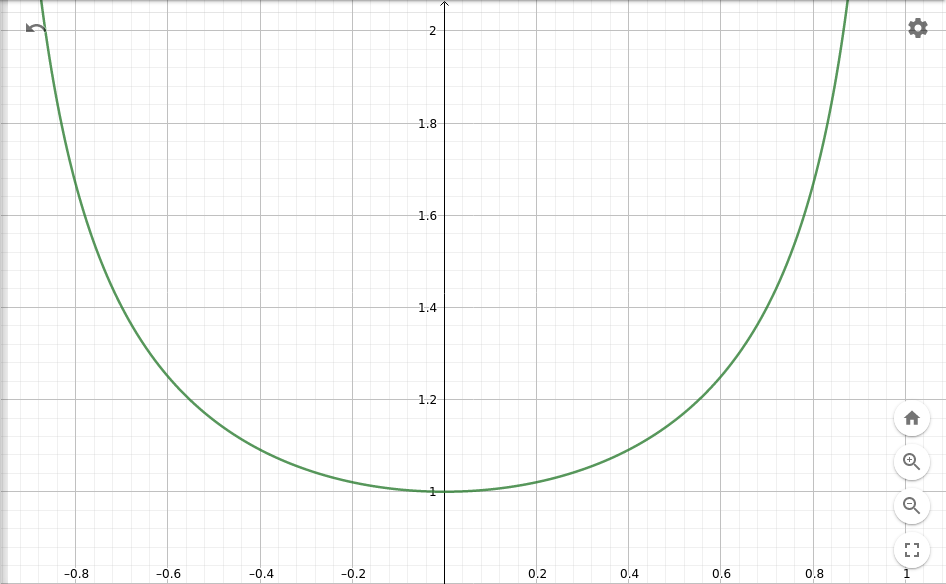
\includegraphics[width=0.4\textwidth]{gamma.png}
\end{wrapfigure}
\subsection{Implikationen}
Dass all diese Effekte nichts mit unserer alltäglichen Erfahrung zu tun haben, liegt an dem Steigungsverhalten von $\gamma$, und der enormen Größen von $c$.
\begin{equation}
c = 299792458 \frac{m}{s}
\end{equation}
Die Parker Solarsonde, eins der schnellsten menschengemachten Objekte, hat eine Geschwindigkeit von etwa $51291 \frac{m}{s} = 1.71 \cdot 10^{-4} c$.
Der Lorentz-Faktor für diese Sonde beträgt $\gamma = 1 + 1.5\cdot10^{-8}$.
Da der Korrekturfaktor durch $\gamma$ bei Geschwindigkeiten, mit denen wir alltäglich zu tun haben, unmessbar ist, erscheinen uns Raum und Zeit nicht relativ.
Dies in Frage zustellen und sich diese Größen als relativ zu veranschaulichen ist extrem schwer.

Deswegen fordert spezielle Relativität unser Vorstellungsvermögen immer wieder heraus.
Dies wird in einer Vielzahl von Paradoxen, deutlich die sich daraus ergeben.
Alle dieser Paradoxen sind mathematisch vergleichsweise einfach zu lösen.

Ein Paradoxon ist zum Beispiel das Tunnel-Paradoxon:
Ein sehr schneller Zug fährt durch ein Tunnel, der kürzer ist als der Zug.
An Eingang und Ende des Tunnels befinden sich Tore, die sehr schnell geöffnet und wieder geschlossen werden können.
Aus der Perspektive einer Person, die neben des Gleisen steht, wird der Zug durch den Lorentz-Faktor verkürzt.
Dadurch können sich die Tore kurz gleichzeitig schließen ohne, dass es zum Unfall kommt.
Aus dem Bezugssystem eines Fahrgasts, wird jedoch der Tunnel gestaucht.
Daher hätte ein gleichzeitiges schließen der Tore zweifellos katastrophale Folgen.
Wie sind diese beiden Beschreibungen vereinbar?
Wir wissen nun aus Abschnitt \ref{trans}, dass Zeit, und somit Gleichzeitigkeit relativ sind.
In dem Beispiel würde der Passant sehen, dass sich die Tore gleichzeitig schließen.
Für den Fahrgast würde sich jedoch erst das eine und dann das andere Tor schließen.

Außerdem ergibt sich unter anderem aus der Gleichung \ref{v}, dass eine Geschwindigkeit größer als $c$ unmöglich ist.
Da dies für alle Objekte gilt, somit auch für Information,  ist dies auch die Geschwindigkeit von Kausalität.
\subsection{Einschränkungen dieses Modells}
Spezielle Relativität beschreibt nur Inertialsysteme in einer flache Raumzeit.
Inertialsysteme sind unbeschleunigt.
Ein Ball, der mit einer Geschwindigkeit gleich 0 losgelassen wird, behält seine Position bei.

Dies löst zum Beispiel das bekannt Zwillingsparadoxon:
Ein Zwilling fährt auf eine Raummission, bei der er, beispielsweise mit halber Lichtgeschwindigkeit, durch das All fliegt, während sein Bruder auf der Erde verbleibt.
Als er zur Erde zurückkehrt, stellt sich die Frage wer nun älter ist.
Nach der speziellen Relativität können sich beide Zwillinge für den Zeitraum der Mission als statisch betrachten, und den anderen als bewegt.
Demnach kommen beide zudem Schluss, dass sie selbst älter sein sollten.

Dabei wird jedoch vernachlässigt, dass der Astronaut beispielsweise zu Alphacentauri fliegt, dort umkehrt und wiederkommt.
Dabei erfährt er eine Beschleunigung, die die spezielle Relativität nicht vorsieht.

Nehme man an der Astronaut führe bei Alphacentauri, ein Swing-by-Manöver durch und ändere so seine Richtung, so würde er sich nicht in einer flachen Raumzeitbewegen.

Diese Überlegung führt uns in die Allgemeine Relativität, die sich maßgeblich von Newtons Gravitation unterscheidet.
Gravitation wird nicht mehr als Kraftfeld beschrieben, sondern als Raumzeitkrümmung, die die inertiale Laufbahn von Objekten verändert.
\newpage
\section{Programm}
Das Programm basiert auf objektorientierter Programmierung und nutzt das pygame Modul, für die graphische Darstellung.

Mit pygame werden, mit gimp selbsterstellte, Linien importiert, um sie rotieren zu können.
Es wird ein Fenster erstellt was die gesamte Grafik enthält.
Außerdem werden Oberflächen für das Diagramm und die Kontrolloberfläche erstellt.
Pygame dient zusätzlich dazu Rechtecke zu erstellen, Kollisionen zu erkennen, die Linien zu rotieren, Schrifteigenschaften zu definieren.
Das Zeichnen wird auch mithilfe von pygame gemacht.

Ich habe ins gesamt vier Klassen entwickelt:.
Eine für die Darstellung der Bezugssysteme im Minkowski-Diagramm, eine für die Darstellung von Buttons und zwei für die Darstellung der Eingabefelder.
Außerdem habe ich jeweils eine Funktion zum wechseln von Bezugssystemen, und zum handhaben von unzulässigen Nutzereingaben erstellt.
\subsection{Nutzung}
Dieses Programm kann in python2.7 und python3 ausgeführt werden.

\textbf{Achtung:} Das Programm importiert die Module \colorbox{gray}{math} und \colorbox{gray}{pygame}.
\colorbox{gray}{pygame} ist in der Regel \underline{nicht} vorinstalliert, ist aber für alle Plattformen leicht und kostenfrei erhältlich.

In dem rechten Feld können Geschwindigkeit und Startposition von Objekten eingeben werden.
Beim klicken der send-Taste, wird die Weltlinie, und die dazugehörige Gleichzeitigkeitslinie des Objektes, in das Koordinatensystem eingezeichnet.
Es können nach belieben Objekte hinzugefügt oder entfernt werden.
Alle sichtbaren Weltlinien können angeklickt werden, um die Lorentz-Transformation in das jeweilige Bezugssystem beobachten zu können.
\\

Zu Beginn läuft einmalig eine Initialisierungsroutine durch.
Pygame wird initialisiert, und dann werden alle globalen Variablen definiert.
Diese sind unter anderem Farben, Fenster, Oberflächen, Bilder, Listen, mathematische Funktionen und textinhalte.

Danach werden die Instanzen der Klassen definiert, die zu Beginn benötigt werden.
Anschließend startet die Hauptschleife.

Sie beginnt damit durch alle pygame-events zu iterieren.
Wird ein 'schließen' Signal erfasst, wird \colorbox{gray}{running} gleich False gesetzt, und das Programm somit beendet.

Innerhalb dieser Schleife werden die pygame-events an alle \colorbox{gray}{handle} Methoden von allen Instanzen übergeben.

Anschließend werden Die Koordinatenachsen gezeichnet, und die \colorbox{gray}{draw} Methoden von allen Instanzen aufgerufen.

Zuletzt werden die Oberflächen auf das Fenster gezeichnet, das Bild erneuert, die Oberflächen zurückgesetzt.
\subsection{Button}
Die Klasse \colorbox{gray}{Button} dient zur Darstellung und Handhabe aller Buttons.
Diese Klasse nimmt einen Typ und optional einen parent als Argument.

In dem Konstruktor wird die Box in Abhängigkeit von Typ definiert.
Anschließend werden weitere Instanzvariablen, für Farbe, Aktivität, Text, Typ, Mutterobjekt definiert.
\subsubsection{Methoden}
Die Methode \colorbox{gray}{handle} wird in der Hauptschleife aufgerufen, und nimmt pygame-Ereignisse als Argumente.
In Abhängigkeit vom Typ wird der Ortsvektor der Maus, an die Oberfläche, angepasst.
Wenn sich die Maus über \colorbox{gray}{self} befindet, wird der Aktivitätszustand auf True gesetzt, andern falls auf False.
Je nach Aktivitätszustand wird in der Methode \colorbox{gray}{draw} die Farbe ändert, was ein Hoverfunktion darstellt.
Wird \colorbox{gray}{self} angeklickt, wird zwischen den Typen unterschieden.
Ist \colorbox{gray}{self.type} gleich 'add', wird der Liste \colorbox{gray}{objs} eine Instanz von \colorbox{gray}{Obj} hinzugefügt.
dabei werden keine Argumente übergeben, wodurch die Standardwerte gelten.

Außerdem wird die Position von \colorbox{gray}{self.rect} angepasst, und es wird Button zum schließen des neuen Feldes erstellt.

Ist \colorbox{gray}{self.type} gleich 'send', wird der Index von \colorbox{gray}{self} ermittelt, und der Methode \colorbox{gray}{enter} übergeben, die in Abschnitt \ref{inputm} näher erläutert wird.

Ist \colorbox{gray}{self.type} gleich 'ok', wird die globale Variable \colorbox{gray}{err} gleich None gesetzt.

Ist \colorbox{gray}{self.type} gleich 'x', wird der Index von \colorbox{gray}{self} ermittelt.
Anschließend wird dieser Index genutzt, um die jeweiligen Einträge in dem Listen \colorbox{gray}{objs}, \colorbox{gray}{delbuttons}, \colorbox{gray}{inputs} und \colorbox{gray}{sendbuttons} zu löschen.
Anschließend werden die Position von den verbleibenden Elementen, sowie der add-Taste angepasst, um das gelöschte Element aufzufüllen.
\\

Die Methode \colorbox{gray}{draw} wird in der Hauptschleife aufgerufen, und zeichnet je nach Typ \colorbox{gray}{self.rect} und \colorbox{gray}{self.txt} auf die passenden Flächen.
\subsection{Input}
Die Klasse \colorbox{gray}{Input} erstellt Eingabefelder, indem sie drei Instanzen der Klasse \colorbox{gray}{Box} erstellt.
Der Sinn dieser Klasse ist, die Liste der Eingabefelder besser zu organisieren, damit Indexe leichter gehandhabt werden können.
\subsubsection{Methoden}
Diese Klasse hat, bis auf den Konstruktor, nur die Methode \colorbox{gray}{enter}, die beim Klicken des 'send' Buttons aufgerufen wird.
Sie prüft die Eingaben in den jeweiligen Feldern auf ihre Zulässigkeit.
Es wird überprüft ob Parameter, die Zahlen sein sollen, Zahlen sind, und, dass keine Geschwindigkeiten über der Lichtgeschwindigkeit eingegeben werden.
Wird eine unzulässige Eingabe erkannt, wird die Funktion \colorbox{gray}{err} aufgerufen, die eine Fallspezifische Fehlermeldung anzeigt.
Sind Felder leer, werden Standardwert ergänzt.
Anschießend wird, mit den ermittelten Parametern, eine neue Instanz von \colorbox{gray}{Obj} erstellt.
\label{inputm}
\subsection{Box}
Die Klasse \colorbox{gray}{Box} ist die eigentliche Maschinerie hinter den Eingabefeldern.
Je nachdem was für Parameter übergeben werden, wird \colorbox{gray}{self} zum Namens-, Positions- oder Geschwindigkeitsfeld.
Demnach werden Position, und Standardinhalt angepasst.
\subsubsection{Methoden}
Die Methode \colorbox{gray}{handle} wird in der Hauptschleife aufgerufen, und nimmt pygame-events als Parameter.
Wird das Feld angeklickt, wird der Standardinhalt entfernt und \colorbox{gray}{self.active} gleich True gesetzt.
Wird woanders hin geklickt, wird \colorbox{gray}{self.active} wieder auf False gesetzt, und gegebenenfalls der Standardinhalt wieder eingesetzt.
Demnach wird auch die Farbe des Feldes angepasst.
Ist anschließend \colorbox{gray}{self.active} True werden die Tastatureingaben gespeichert.
\\

\colorbox{gray}{draw} zeichnet dann den passenden Text und das Felde in der richtigen Farbe.
\subsection{Obj}
\colorbox{gray}{Obj} ist das Herzstück des Programms.
Es handhabt alle Einträge in das Diagramm.
Es nimmt Argumente, die den Namen, den Index, die Position, die Geschwindigkeit, den Farbindex und t = 0 definieren.
Es werden zunächst alle Argumente als Instanzvariablen gespeichert.
Anschließend werden der Winkel der Weltlinien und die Weltlinie definiert.
Danach wird \colorbox{gray}{pos} definiert, was das errechnen von Punkten entlang der Weltlinie massiv erleichtert.
Falls der Betrag von \colorbox{gray}{self.v} kleiner als 1 ist, werden zusätzliche graphische Features definiert.
Diese sind die Gleichzeitigkeitslinie für t=0, kleine Einheitsmarker für x und t und das gesamte Koordinatensystem für das jeweilige Bezugssystem.

Für die Gleichzeitigkeitslinie wird eine neue Linie erstellt, die um 90-\colorbox{gray}{self.angle} rotiert ist.
Für die Einheitsmarker wird der Schnittpunkt zwischen den beiden Gerade ermittelt.
Von dort ausgehend werden iterativ neue Positionen für Marker entlang der Geraden ermittelt die um eine Konstante $\cdot \gamma$ von einander entfernt sind.

Ähnlich wird auch das Koordinatensystem definiert.
Hier wird jedoch der Referenzpunkt der Geraden als Startpunkt gewählt.

Zuletzt wird die Position des Namens definiert.
Der Name steht immer rechts neben der Weltlinie soweit oben wie es möglich ist, ohne, dass zwei Namen kollidieren.
\subsubsection{Methoden}
\colorbox{gray}{draw} prüft ob \colorbox{gray}{self.v} gleich 1 ist.
Wenn das der Fall ist, wird nur die Weltlinie gezeichnet.
Andernfalls werden mindestens die Einheitsmarker, und die Gleichzeitigkeitslinie hinzugefügt.
Ist \colorbox{gray}{self.active} True, wird zusätzlich noch das gesamte Koordinatensystem gezeichnet.
\\

\colorbox{gray}{handle} handhabt das Nutzerverhalten in Bezug auf das Diagramm.
Befindet sich die Maus über der Weltlinie, wird \colorbox{gray}{self.active} zu True.
Wir die Weltlinie angeklickt, wird die Funktion \colorbox{gray}{change} aufgerufen, und somit das wechseln des Bezugssystem initiiert.
Wie das Funktioniert ist in Abschnitt \ref{func} näher erklärt.
\subsection{Funktionen}
\label{func}
Die Funktion \colorbox{gray}{error} wird von der Funktion \colorbox{gray}{enter} bei jedem Fehlerfall aufgerufen.
Es wird ein Fallspezifischer Fehlerwert übergeben.
Die Funktion error erstellt ein Fenster, auf dem eine fehlerspezifische Nachricht angezeigt wird.
Außerdem wir ein 'ok' Button erstellt, mit dem das Fenster wieder geschlossen werden kann.
\\

Die Funktion \colorbox{gray}{change} wird aufgerufen, wenn der Nutzer eine Weltlinie anklickt, und danach in jeder Iteration des Programms, bis die Lorentz-Transformation fertig ist.
Sie nimmt den Index des gewünschten Bezugssystems als Argument.
Die Änderung der Bezugssystems wird, der anschaulichkeitshalber für jede Größe nacheinander gemacht.
Zuerst wird endlang der x-Achse verschoben, dann wird die Geschwindigkeit angepasst und zuletzt t justiert.
Dies alles wird aber nicht in Schleifen in der Funktion gemacht, da so die zwischenschritte zur fertigen Transformation nicht gezeichnet werden würden.
\section{Quellen}
\url{https://stackoverflow.com/questions/46390231/how-to-create-a-text-input-box-with-pygame}
\url{https://www.youtube.com/playlist?list=PLD9DDFBDC338226CA}
\url{https://www.youtube.com/playlist?list=PLDB7DB12B34395EC5}
\url{https://www.pygame.org/docs/}
\url{https://en.wikipedia.org/wiki/Special_relativity}
\url{http://edu-observatory.org/olli/Relativity/Minkowski_diagram.png}
\end{document}
